\begin{starred}
\section{实验:研究液体的压强和深度的关系}\label{sec:5-6}
\end{starred}

\begin{wrapfigure}[12]{r}{4.5cm}
    \centering
    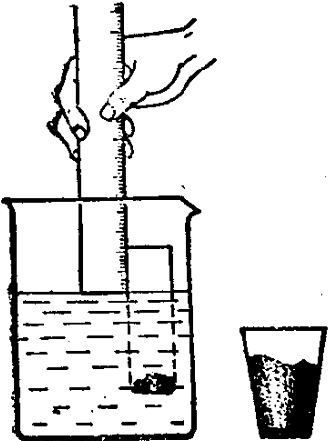
\includegraphics[width=4cm]{../pic/czwl1-ch5-20}
    \caption{}\label{fig:5-20}
\end{wrapfigure}

上面讲了液体的压强是随深度的增加而增加的。现在我们用实验来进一步研究液体的压强随深度而变化的规律。

在这个实验里,液体内部的压强是利用一个平底玻璃管来测量的:往这个坡璃管里装些细沙,使它竖直浮在水中不动(图 \ref{fig:5-20})。
这时它在竖直方向上受到两个力的作用,一个是向下的重力,一个是水对管底向上的压力,这两个力大小相等。
所以称出管和沙受到的重力就知道了水对管底向上的压力,再测出管底的面积,就可以算出压强。

\shiyan{目的} 研究液体的压强和深度的关系。

\shiyan{器材} 天平,平底玻璃管,烧杯〈内装适量的水),细沙,三角板,刻度尺,角匙。

\shiyan{步骤}

(1) 用刻度尺量出玻璃管的高度。用刻度尺和三角板量出管的外径,算出管底的面积。

(2) 用角匙把少量细沙装入玻璃管中,设法使管竖直地浮在水中。用刻度尺量出玻璃管顶部到水面距离。
用管的高度减去这个距离,算出管底浸入水中的深度。

(3) 从水中取出玻璃,擦干后用天平称出玻璃管和沙的质量,算出它们受到的重力。

(4) 向玻璃管里加一些细沙,把上面的实验重一次。再向管里加一些细沙,把实验再做一次。

(5) 把测出的和算出的数据填入下表。

\begin{table}[H]
    \centering
    \begin{tabular}{|w{c}{4em}|w{c}{4em}|*{5}{w{c}{5em}|}}
        \hline
        \tabincell{c}{实验\\次数} & \tabincell{c}{玻璃\\管高\\(米)} & \tabincell{c}{玻璃管顶部\\到水面的距\\离(米)} & \tabincell{c}{玻璃管底浸\\入水中的深\\度(米)} & \tabincell{c}{玻璃管和沙\\重 $G = mg$ \\(牛顿)} & \tabincell{c}{玻璃管底\\的面积\\($\pfm$)} & \tabincell{c}{水对玻璃管\\底的压强\\(帕斯卡)}  \\ \hline
        1 & & & & & & \\ \hline
        2 & & & & & & \\ \hline
        3 & & & & & & \\ \hline
    \end{tabular}
\end{table}


(6) 利用求得的压力和管底的面积算出水对管底的压强。

(7) 根据三次实验的结果,研究一下液体的压强和深度是不是成正比。

% \begin{wrapfigure}[12]{r}{4.5cm}
%     \centering
%     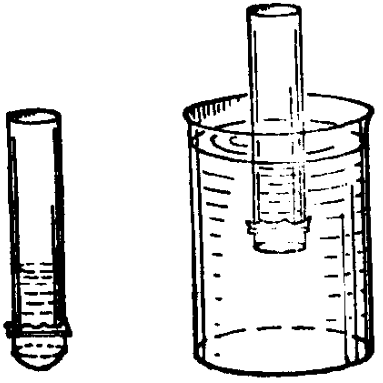
\includegraphics[width=4cm]{../pic/czwl1-ch5-21}
%     \caption{}\label{fig:5-21}
% \end{wrapfigure}


\lianxi

(1) 水坝的下部为什么要比上部修得厚?

(2) 潜水艇潜入水下的深度有一定的限度,潜入水下过深,艇壳就可能损坏,这是为什么?

(3) 图 \ref{fig:5-21} 中玻璃管的下端扎有橡皮膜,管里装着有色的水,这时橡皮膜向下凸出。
把玻璃管管外的水面跟管内的水面相平时,橡皮膜就变平。这是为什么?

\begin{figure}[htbp]
    \centering
    \begin{minipage}{5cm}
    \centering
    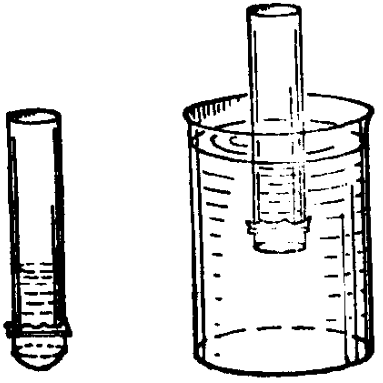
\includegraphics[width=5cm]{../pic/czwl1-ch5-21}
    \caption{}\label{fig:5-21}
    \end{minipage}
    \qquad
    \begin{minipage}{9cm}
    \centering
    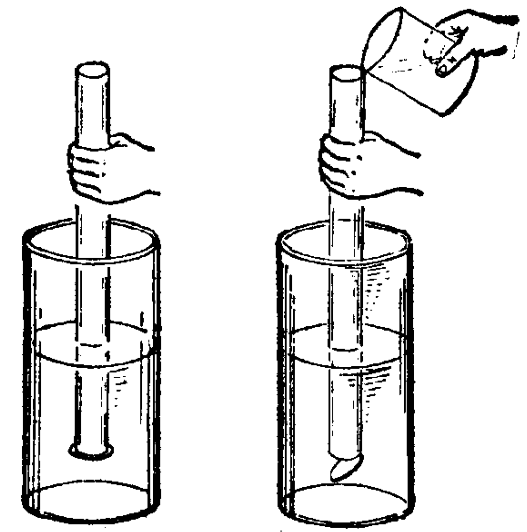
\includegraphics[width=6cm]{../pic/czwl1-ch5-22}
    \caption{}\label{fig:5-22}
    \end{minipage}
\end{figure}


\nonumsection{小实验:研究液体的压强}

找一个两端开口的玻璃管,用塑料片(或硬纸片)挡住下端管口,用手按住塑料片,把玻璃管竖直插入水槽里,
松开手后,塑料片并不下沉(图 \ref{fig:5-22}), 为什么?
用一个杯子把水沿管壁缓缓地倒入管内,注意观察管内水面达到多高时塑料片才会下沉。说明塑料片这时下沉的原因。

% \begin{figure}[htbp]
%     \centering
%     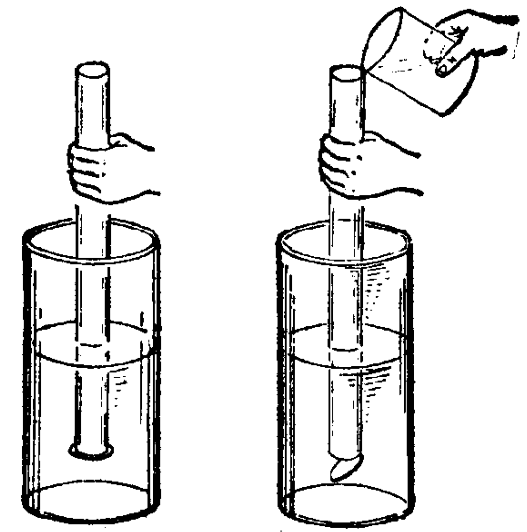
\includegraphics[width=0.4\textwidth]{../pic/czwl1-ch5-22}
%     \caption{}\label{fig:5-22}
% \end{figure}

